\documentclass[a4paper]{article}
\usepackage{ctex}
\usepackage{geometry}
\usepackage{amsmath}
\usepackage{ulem}
\usepackage{graphicx}
\usepackage{siunitx}
\usepackage{enumitem}
\usepackage{multirow}
\usepackage{adjustbox}
\usepackage[hidelinks]{hyperref}
\usepackage{tabularx}
\usepackage{array}
\newcolumntype{Y}{>{\centering\arraybackslash}X}

\geometry{left=2.5cm, right=2.5cm, top=2.5cm, bottom=2.5cm}
\zihao{-4}

\begin{document}

\noindent\textbf{班级：24级整合科学班} \hspace{1cm} \textbf{学号：2400017802} \hspace{1cm} \textbf{姓名：冯翊展} \hspace{1cm} \textbf{评分：}\\
\textbf{同组学生：胡家豪} \\
\textbf{实验名称：流体中的运动以及低雷诺数下的生命}   \hfill \textbf{实验日期：2025年2月21/28日} 

\hrule
\vspace{3mm}

\begin{enumerate}[label=\chinese*.,left=0pt]
    \item 实验目的
    \\[3mm]
    通过观察比较不同尺寸与材质的金属珠落入甘油和水中的运动情况，来模拟物体在高、低雷诺数流体中的运动体系特性，从而体会微观尺度上惯性力和粘性力的作用，以及细菌等生物的运动特征。
    
    \item 实验内容
    \begin{enumerate}[label=\arabic*.,left = 0pt]
        \item 低雷诺数：在甘油中测量4种不同尺寸的铝珠下落的垂直速度，使用相机记录实验数据并进行数据分析，依据下落速度估算不同小球下落时的雷诺数，并与理论预测结果对比。
        \item 高雷诺数：在水中测量4种不同尺寸的钢珠下落的垂直速度，使用相机录制视频，使用 ImageJ 软件进行数据分析和计算，依据下落速度估算不同小球下落时的雷诺数，并于理论预测结果对比
    \end{enumerate}
    
    \item 基本原理
    \begin{enumerate}[label=\arabic*.,left = 0pt]
        \item 雷诺数（$R$）是衡量惯性力与粘性力的比值，定义为：
        \begin{equation}
            \label{tab:Reynold}
            R=\frac{\rho a v}{\eta}
        \end{equation}
        其中 $\rho$ 是流体密度，$v$ 是物体速度，$a$ 是物体的特征长度，$\eta$ 是流体的（动态）粘度。

        \item 低雷诺数下，物体运动受到的阻力符合斯托克斯阻力定律：
        \begin{equation}
            \label{tab:Stokes}
            F_d=6 \pi \eta r v
        \end{equation}
        物体到达终速 $v_{\text{term}}$ 时，
        \begin{equation}
            \label{tab:vterm1}
            v_{\text{term}} = \frac{M'g}{6\pi \eta r} =\frac{\frac{1}{6}d^3(\rho_{\text{铝}}-\rho_{\text{甘}})g}{3\pi\eta d} = \frac{(\rho_{\text{铝}}-\rho_{\text{甘}})g}{18\pi\eta }d^2
        \end{equation}
        其中 $M'$ 是扣除浮力的物体有效质量。

        \item 一个落在充满液体的圆筒的中心的物体下落速度可以通过以下公式修正：
        \begin{equation}
        \label{tab:corr}
            v_{\text{corr}} = \frac{v_{\text{meas}}}{1-2.10(d/D)+2.09(d/D)^3}
        \end{equation}
        其中，$v_{\text{meas}}$ 是实验测得的终速，$d$ 是球体的直径，$D$ 是量筒直径，$v_{\text{corr}}$ 是球体落在无界流体中终速的预期值。

        \item 高雷诺数下，物体运动受到的阻力符合公式：
        \begin{equation}
            \label{tab:drag}
            F_d=\frac{1}{2} \rho C_d A v^2
        \end{equation}
        其中 $C_d$ 是阻力系数，$A$ 是物体的横截面积。物体达到终速 $v_{\text{term}}$ 时，
        \begin{equation}
            \label{vterm2}
            v_{\text{term}}=\sqrt{\frac{2M'g}{\rho C_d A}} = \sqrt{\frac{2\cdot \frac{1}{6}d^3(\rho_{\text{铁}}-\rho_{\text{水}})g}{\rho_{\text{水}}C_d\frac{1}{4}\pi d^2}}=\sqrt{\frac{4(\rho_{\text{铁}}-\rho_{\text{水}})g}{3\pi\rho_{\text{水}}C_d}}d^{\frac{1}{2}}
        \end{equation}
    \end{enumerate}
    
    \item 仪器与试剂
    \begin{enumerate}[label=\textbullet,left = 0pt]
        \item 流体：水、甘油
        \item 固体球：铝珠（直径 \qty{4}{\milli \m}、\qty{6}{\milli \m}、\qty{8}{\milli \m}、\qty{10.4}{\milli \m}）、钢珠（直径 \qty{4}{\milli \m}、\qty{6}{\milli \m}、\qty{8}{\milli \m}、\qty{10}{\milli \m}）
        \item 测量工具：量筒（\qty{100}{\milli \litre}、\qty{250}{\milli \litre}）、秒表、尺子
        \item 数据采集与分析设备：相机、电脑（配有 ImageJ 和 Matlab 软件）
    \end{enumerate}
    
    \item 实验步骤
    \begin{enumerate}[label=\Alph*., left = 0pt]
        \item 低雷诺数
            \begin{enumerate}[label=\arabic*.,left = 0pt]
                \item 使用 \qty{100}{\milli \L}量筒量取 \qty{100}{\milli L} 甘油，选取不同尺寸的铝珠，接近液面沿量筒中心投入甘油中。
                \item 测量铝珠从一个 \qty{10}{\milli \L} 标记到另一个所需的时间，用尺子测量珠子走过的距离，并计算铝珠在甘油中的终速。
                \item 记录多次测量结果，计算平均值及标准差。
                \item 测量量筒直径，校正壁效应对速度的影响，并计算雷诺数。
                \item 在 Matlab 中绘制终速与半径的曲线，并进行线性拟合分析。
            \end{enumerate}

        \item 高雷诺数
            \begin{enumerate}[label=\arabic*., left = 0pt]
                \item 使用 \qty{250}{\milli \L}量筒量取 \qty{250}{\milli L} 水，选取不同尺寸的钢珠，接近液面沿量筒中心投入水中。
                \item 使用使用高速连拍功能采图，测量两条刻度线之间的像素距离，并使用之前测得的实际距离，获得像素与厘米的转换比例。
                \item 将图像导入 ImageJ，用珠子在一次曝光时间里下落的距离除以曝光时间计算速度。记录多次测量结果，计算平均值及标准差。
                \item 校正壁效应与阻力系数对速度的影响，并计算雷诺数。
                \item 在 Matlab 中绘制终速与半径的曲线，并进行线性拟合分析。
            \end{enumerate}
    \end{enumerate}
    
    
    \item 实验结果与分析
    \begin{enumerate}[label=\Alph*., left=0pt]
        \item 低雷诺数 \\
        \textbf{数据分析：}实验首先采用秒表手计的方法测定四种直径（$d$）的铝珠垂直落入甘油后在量筒中下落一个 \qty{10}{\milli \m} 刻度的时间（$t$），进而计算得到铝珠下落的终速。测得实验数据如表~\ref{tab:data_1} 所示，其中部分数据点因计时失误而舍去。\\[-7mm]
        \begin{table}[h]
            \caption{四种尺寸的铝珠落入甘油中的终速测定}
            \label{tab:data_1}
            \centering
            \scalebox{0.9}{ 
            \setlength{\tabcolsep}{3pt}
            \renewcommand{\arraystretch}{1.2} 
            \begin{tabular}{|>{\centering\arraybackslash}m{1.2cm}|*{16}{c}|} 
                \hline
                \multicolumn{1}{|c|}{$d$/\si{\milli\metre}} & \multicolumn{16}{c|}{$t$/\si{\second}} \\ \hline
                \multirow{2}{*}{4}  & 2.33 & 2.13 & 2.11 & 2.30 & 2.21 & 2.16 & 2.26 & 2.23 & 2.25 & 2.20  & 2.30  & 2.35 & 2.20  & 2.33 & 2.31 & 2.36 \\ 
                & 2.08 & 2.23 & 2.09 & 2.26 & 2.23 & 2.11 & 2.25 & 2.23 & 2.18 & 2.18 & 2.18 & 2.21 & 2.18 & 2.20  & 2.25 & 2.26 \\ \hline
                \multirow{2}{*}{6}  & 1.21 & 1.10 & 1.26 & 1.11 & 1.28 & 1.25 & 1.15 & 1.18 & 1.10  & 1.26 & 1.33 & 1.13 & 1.20  & 1.13 & 1.18 & 1.15 \\ 
                & 1.30  & 1.13 & 1.18 & 1.21 & 1.13 & 1.21 & 1.06 & 1.11 & 1.23 & 1.11 & 1.21 & 1.34 &      &      &      &      \\ \hline
                \multirow{2}{*}{8}  & 1.05 & 0.76 & 0.70  & 0.78 & 0.83 & 0.95 & 0.83 & 0.91 & 0.78 & 1.00 & 0.96 & 0.80  & 0.86 & 0.83 & 0.83 & 0.75 \\ 
                & 0.93 & 0.76 & 0.88 & 0.86 & 0.90  & 0.86 & 0.86 & 0.73 & 0.80  & 0.78 & 0.78 & 0.91 & 0.80  & 1.00  &      &      \\ \hline
                \multirow{2}{*}{10.4}& 0.56 & 0.63 & 0.56 & 0.66 & 0.53 & 0.56 & 0.71 & 0.60  & 0.60  & 0.65 & 0.63 & 0.70  & 0.71 & 0.66 & 0.63 & 0.68 \\ 
                & 0.61 & 0.64 & 0.68 & 0.63 & 0.60  & 0.68 & 0.61 & 0.61 & 0.73 & 0.63 & 0.61 & 0.66 & 0.66 &      &      &      \\ \hline
            \end{tabular}
        }
        \end{table}

        实际测得 \qty{100}{\milli \L}的量筒每两个 \qty{10}{\milli \L}之间的数值间距为 \qty{0.0150}{\m}，量筒的直径（$D$）为 \qty{0.0291}{\m}；实验所用铝珠密度 $\rho_{\text{铝}}= \qty{2.70}{\g \per \cm \cubed}$，甘油密度为 $\rho_{\text{甘}}= \qty{1.26}{\g \per \cm \cubed}$；实验时室温为 \qty{20.7}{\degreeCelsius}，甘油黏度 $\eta = \qty{1333}{\centi P}$。据此分别计算四种尺寸的铝珠每次下落的平均终速（$v_{\text{meas}}$）， 并引入式~\eqref{tab:corr} 修正壁效应对终速的影响，得到相应的修正值（$v_{\text{corr}}$）；使用~\eqref{tab:Reynold} 式计算相应的雷诺数（$R$）；使用~\eqref{tab:vterm1} 式计算铝珠的理论终速（$v_{\text{term}}$）。
        计算结果统一见表~\ref{tab:data_2}:
        \\[-8mm]
        \begin{table}[h]
            \caption{四种尺寸的铝珠实际终速与理论终速对比}
            \label{tab:data_2}
            \centering
            \scalebox{1}{ 
            \setlength{\tabcolsep}{3pt}
            \renewcommand{\arraystretch}{1.2} 
            \begin{tabular}{|c|c|c|c|c|c|}
            \hline
            $d$/\qty{e-3}{\m} & $v_{\text{meas}}/\qty{e-3}{\m \per\s}$  & $\sigma/ \qty{e-3}{\m \per \s}$ & $v_{\text{corr}}/ \qty{e-3}{\m \per \s}$  & $v_{\text{term}} / \qty{e-3}{\m \per \s}$  & $R / \qty{e-3}{}$  \\ \hline
            4       & 6.75 & 0.22     & 9.42 & 9.41 & 25.5 \\ \hline
            6       & 12.7 & 0.77     & 21.7 & 21.2 & 71.9 \\ \hline
            8       & 17.8 & 1.7      & 38.3 & 37.6 & 135  \\ \hline
            10.4    & 23.8 & 1.8      & 68.9 & 63.6 & 234  \\ \hline
            \end{tabular}
            }
        \end{table}
        \\
        经过壁效应修正，实际测量结果与使用斯托克斯公式预测值有较好的符合。计算得到的雷诺数均小于$1$，符合低雷诺数的情况
        
        采用Matlab绘制终速对半径的曲线如左图，进一步取对数作图如右图：
        \begin{figure}[h]
            \centering
            \begin{minipage}{0.47\textwidth}
                \centering
                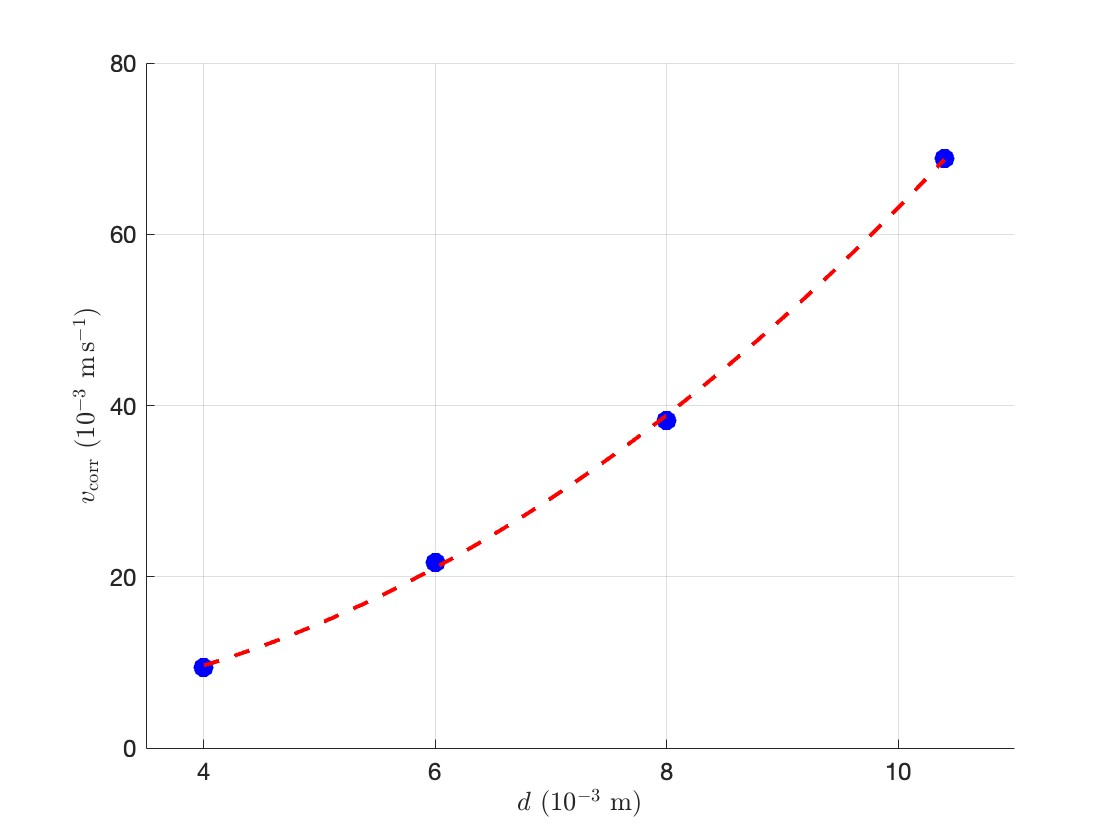
\includegraphics[width=\textwidth]{Fig_1.jpg}
                \caption{$v_\text{corr}-d$ 曲线}
            \end{minipage}
            \begin{minipage}{0.47\textwidth}
                \centering
                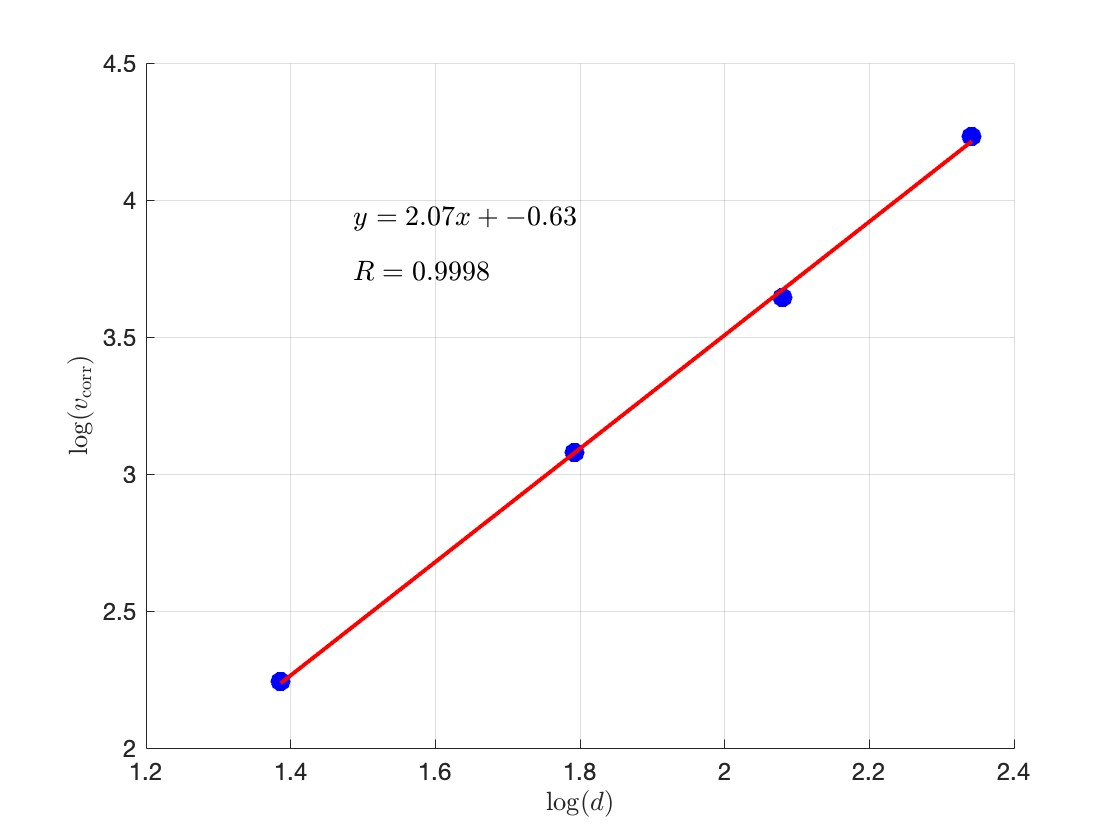
\includegraphics[width=\textwidth]{Fig_2.jpg}
                \caption{$\log(v_{\text{corr}})-\log(d)$ 曲线}
            \end{minipage}
        \end{figure}
        \\
        其中斜率 $k=2.07\approx2$，基本符合低雷诺数下的理论预期。
        
        \textbf{误差分析：}实验主要的随机误差来源于观察角度与计时的方式：我们采取观察铝珠下落经过量筒刻度线并手动计时的方式测量终速，由于无法保证观察角度以及反应速度始终保持一致，这种测量方式具有较大误差。实验的系统误差则主要来源于甘油密度与黏度变化：实验中使用了多组甘油样品，其中部分甘油含气泡较多，并存在吸水情况，随着时间推移其密度与黏度逐渐下降，同时气泡的存在也会减少小球与甘油的接触面积，这将导致甘油对铝珠的粘滞力减小，铝珠的实际终速高于理论预测，这也符合实验事实。
        \item 低雷诺数 \\
        \textbf{数据分析：}与低雷诺数情况的分析方法类似，我们分别对四种尺寸的钢球测定其下落终速及标准差，引入式~\eqref{tab:corr} 修正壁效应对终速的影响，并使用~\eqref{tab:Reynold} 式计算相应的雷诺数（$R$）。计算结果见表~\ref{tab:data_3}。
        \begin{table}[h]
            \caption{四种尺寸的钢珠实际终速与理论终速对比}
            \label{tab:data_3}
            \centering
            \renewcommand{\arraystretch}{1.2}
            \setlength{\tabcolsep}{3pt}
            \scalebox{1}{
                \begin{tabularx}{0.8\linewidth}{|Y|Y|Y|Y|Y|}
                \hline
                $d$/\qty{}{\m} & $v_{\text{meas}}/\qty{}{\m \per\s}$  & $\sigma/ \qty{}{\m \per \s}$ & $v_{\text{corr}}/ \qty{}{\m \per \s}$ & $R \qty{}{}$  \\ \hline
                0.004	& 1.24 & 0.0872	  & 1.50 & 5990  \\ \hline
                0.006	& 1.34 & 0.0522	  & 1.81 & 10833  \\ \hline
                0.008	& 1.40 & 0.0334	  & 2.13 & 17002  \\ \hline
                0.010   & 1.45 & 0.0346   & 2.50 & 24957 \\ \hline
                \end{tabularx}
            }
        \end{table} 
        \\
        从表中看到，所有情况下的雷诺数均大于$5000$，属于高雷诺数的情况，且小球直径越大，其下落速度越快，雷诺数越大。进一步作图得到斜率为 $0.55$, 与公式预测的 $0.5$ 基本吻合。
        \begin{figure}[h]
            \centering
            \begin{minipage}{0.47\textwidth}
                \centering
                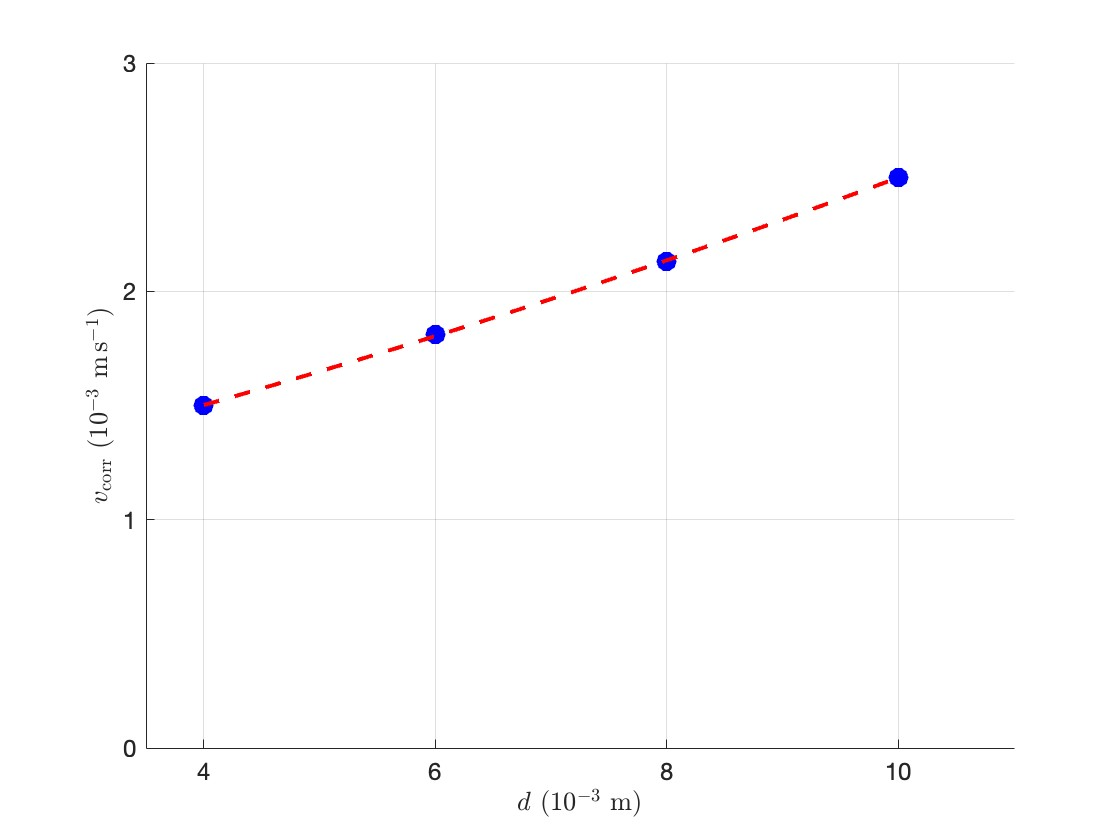
\includegraphics[width=\textwidth]{Fig_3.jpg}
                \caption{$v_\text{corr}-d$ 曲线}
            \end{minipage}
            \begin{minipage}{0.47\textwidth}
                \centering
                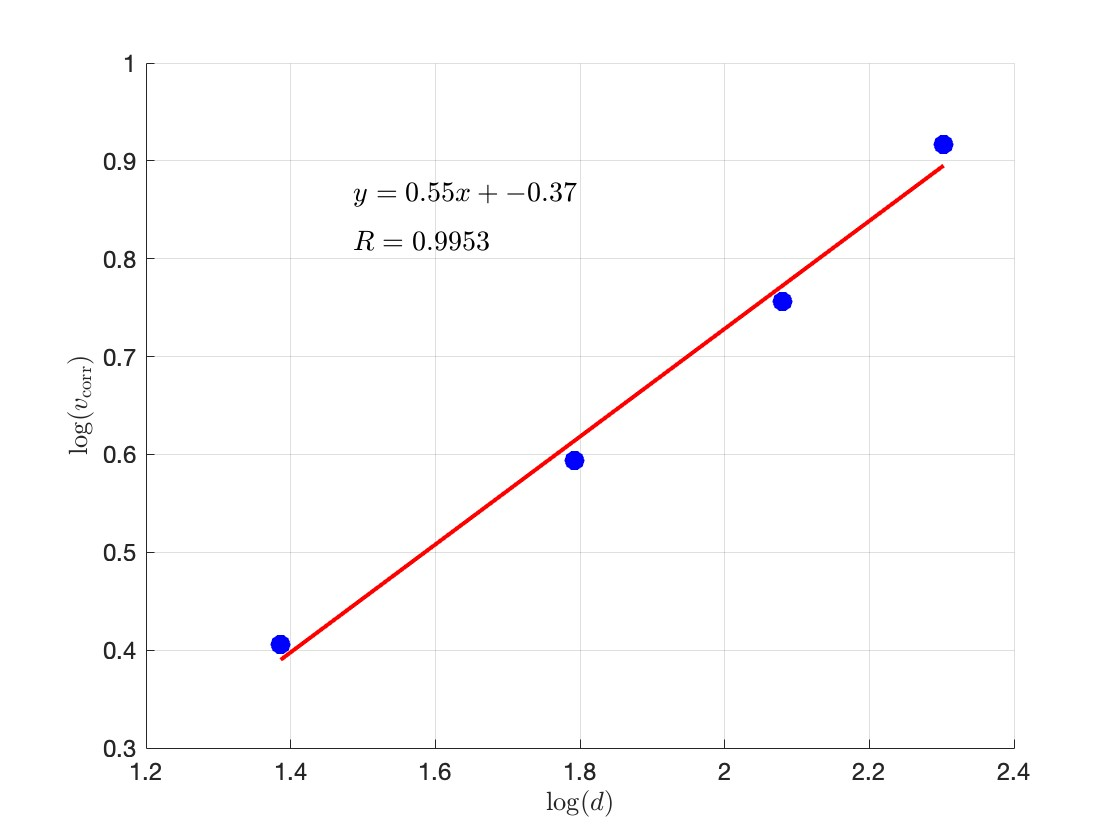
\includegraphics[width=\textwidth]{Fig_4.jpg}
                \caption{$\log(v_{\text{corr}})-\log(d)$ 曲线}
            \end{minipage}
        \end{figure}
        
        \textbf{误差分析：}首先，相较于在甘油中下落，钢珠在水中下落速度较快，较难判断铁球是否达到匀速状态，可能使得所测速度偏低；其次，在释放钢球的过程中，无法保证每次小球初始位置都恰好位于量筒中心，且其轨迹并不一定是竖直直线，因此壁效应修正公式未必准确适用；另外，本实验录制的视频帧数较低，无法准确观察钢珠重心的精确位置，尤其是尺寸较小的钢珠，因此从表中也可看出，钢珠尺寸越小，标准差反而越大。
    \end{enumerate}




    
    \item 思考题
    \begin{enumerate}[label=\arabic*.,left = 0pt]
        \item 雷诺数的单位是什么？请附推导过程。
        \\[2.5mm]
        解：雷诺数可表达为：
        $$R=\frac{\rho a v}{\eta}.$$
        代入单位进行量纲分析：
        $$(R)=\frac{\si{\kg \per \m \cubed \cdot \si{\m} \cdot \si{\m \per \s}}}{\si{\Pa \cdot \s}} = \frac{\si{\kg \per \m \cubed \cdot \si{\m} \cdot \si{\m \per \s}}}{\si{\kg \per (\m \cdot \s)}} = 1.$$
        故雷诺数无量纲。
    
        \item 使用引言部分给出的参数，计算一个在水中游动的细菌的雷诺数，并估算一个人在游泳时的雷诺数（$\rho_{\text{水}} = \qty{1}{\g \per \cm \cubed}$，$\eta_{\text{水}} = \qty{1}{cP}$，$\si{cP}$ 代表厘泊，即百分之一泊，$1$ 泊等于 $\qty{1d-1}{\Pa\s}$）。
        \\[2.5mm]
        解：对于细菌，$a\approx\qty{1}{\micro \metre}$，$v \approx \qty{20}{\micro \metre \per \second}$，故其雷诺数为：
        $$R=\frac{\qty{1}{\gram \per \cm \cubed} \cdot \qty{1}{\micro \metre} \cdot \qty{20}{\micro \metre \per \second}}{1\cdot 10^{-3} \qty{}{\Pa \second}}=2\cdot 10^{-5}.$$
        对于人，$a\approx \qty{1.8}{\m}$，$v\approx \qty{1.5}{\m \per \s}$，故其雷诺数为：
        $$R=\frac{\qty{1}{\gram \per \cm \cubed} \cdot \qty{1.8}{\metre} \cdot \qty{1.5}{\metre \per \second}}{1\cdot 10^{-3} \qty{}{\Pa \second}}=2.7 \cdot 10^6.$$
    
        \item 证明在低雷诺数下，珠子落入流体中的终速与其半径的平方成正比（使用斯托克斯阻力定律）。
        \begin{equation*}
            v_{\text{term}} \propto r^2
        \end{equation*}
        提示：从 $M' g = 6\pi r \eta v_{\text{term}}$ 开始推导，并以 $r$ 作为单位展开。
        \\[2.5mm]
        证明：
        $$M'g = (\rho_{\text{珠}}-\rho_{\text{水}}) \cdot \frac{4}{3} \pi r^3 g = 6\pi r \eta v_{\text{term}} \implies v_{\text{term}}= \frac{2(\rho_{\text{珠}}-\rho_{\text{水}})g}{9\eta} r^2 \propto r^2$$

        \item 证明在高雷诺数下，珠子落入流体中的终速与其半径的平方根成正比。
        \begin{equation*}
            v_{\text{term}} \propto r^{1/2}
        \end{equation*}
        提示：从 $M' g = \frac{1}{2} \rho C_d A v_{\text{term}}^2$ 开始推导，并以 $r$ 作为单位展开。
        \\[2.5mm]
        证明：
        $$M'g = (\rho_{\text{珠}}-\rho_{\text{水}}) \cdot \frac{4}{3} \pi r^3 g = \frac{1}{2} \rho C_d A v_{\text{term}}^2 = \frac{1}{2} \rho C_d \pi r^2 v_{\text{term}}^2$$
        $$\implies v_{\text{term}}= \sqrt{\frac{8(\rho_{\text{珠}}-\rho_{\text{水}})g}{3\rho C_d}} r^{1/2} \propto r^{1/2}$$

        \item 运动方程 14 可以使用分离变量法来求解，方程原形式为：
        \begin{equation*}
            m \frac{\mathrm{d}v}{\mathrm{d}t} = mg - bv
        \end{equation*}
        将所有 $v(t)$ 项移至方程一侧，所有 $t$ 项移至另一侧，我们得到：
        \begin{equation*}
            \frac{\mathrm{d}v}{g-\left(\frac{b}{m}\right) v} = \mathrm{d}t
        \end{equation*}
        积分并解出 $v(t)$，至于积分常数，令初始条件为 $v(0) = 0$。
        \\[2.5mm]
        解：对等式两边积分，得到：
        $$\int \frac{\mathrm{d}v}{g- \left(\frac{b}{m}\right)v}= -\frac{m}{b} \ln \left( g- \frac{b}{m}v \right) = t+C$$
        $$\implies v(t) = \frac{m}{b} \left[g-e^{-\frac{b}{m}(t+C)}\right].$$
        又，$v(0)=0 \implies g-e^{-\frac{b}{m}C} = 0$，故
        $$v(t) = \frac{m}{b} \left(g-ge^{-\frac{b}{m}t}\right)= \frac{mg}{b}\left(1-e^{-\frac{b}{m}t} \right).$$
    \end{enumerate}
\end{enumerate}



\end{document}